\documentclass[tikz,border=5pt]{standalone}

\usepackage{tikz}
\usepackage{pgfplots}
\pgfplotsset{compat=1.17}

\begin{document}
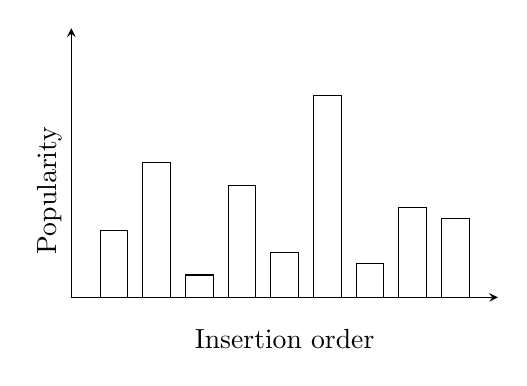
\begin{tikzpicture}
\begin{axis}[
    width=7cm, height=5cm,
    axis lines=middle,
    xtick=\empty,
    ytick=\empty,
    xmin=0, xmax=10,
    ymin=0, ymax=1.2,
    xlabel={Insertion order},
    ylabel={Popularity},
    xlabel style={
      at={(axis cs:5,0)},
      anchor=north,       % 'north' will put text below that point
      yshift=-8pt         % shift more or less as needed
    },
    ylabel style={
      at={(axis cs:0,0.6)},
      rotate=90,
      anchor=south,       % 'south' puts the rotated text to the left of that point
      xshift=-10pt        % shift more or less as needed
    },
]
    \addplot[ybar, fill=white, draw=black] coordinates {
        (1,0.3)
        (2,0.6)
        (3,0.1)
        (4,0.5)
        (5,0.2)
        (6,0.9)
        (7,0.15)
        (8,0.4)
        (9,0.35)
    };
\end{axis}
\end{tikzpicture}
\end{document}